%\documentclass{amsart}

\documentclass{article}
\usepackage[letterpaper,hmargin=15mm,vmargin=20mm]{geometry}
\usepackage[nosetup, colorlinks]{tony}
\usepackage{graphicx}

\usepackage{amsmath,amssymb}
\usepackage{siunitx}

\usepackage{mathpazo}
\usepackage{microtype}
\usepackage{multicol}

\usepackage{diagbox}

\usepackage{color}
\usepackage[dvipsnames]{xcolor}
%\usepackage[printwatermark]{xwatermark}
%\newwatermark*[allpages,color=gray!50,angle=45,scale=3,xpos=0,ypos=0]{DRAFT}

\usepackage{tikz}
\usetikzlibrary{arrows}

\DeclareMathOperator{\sgn}{sgn}
\DeclareMathOperator{\NLL}{NLL}
\newcommand{\sind}[1]{^{(#1)}}

\title{6.867: Problem Set 3}
\date{November 10, 2016}

\begin{document}
\maketitle

\begin{multicols}{2}

% % % % % % % % % %
%    PROBLEM 1
% % % % % % % % % %

\section{Neural Networks}
\label{sec:nn}

\def\layersep{2.5cm}

% tikz taken and adjusted from
% http://www.texample.net/tikz/examples/neural-network/
\begin{figure*}[t]
    \label{fig:samplenn}
    \centering
    \begin{tikzpicture}[shorten >=1pt,->,draw=black!50, node distance=\layersep]
        \tikzstyle{every pin edge}=[<-,shorten <=1pt]
        \tikzstyle{neuron}=[circle,fill=black!25,minimum size=16pt,inner sep=0pt]
        \tikzstyle{input neuron}=[neuron, fill=CornflowerBlue!50];
        \tikzstyle{output neuron}=[neuron, fill=Dandelion!50];
        \tikzstyle{hidden neuron}=[neuron, fill=YellowGreen!50];
        \tikzstyle{annot} = [text width=5em, text centered]
    
        % Draw the input layer nodes
        \foreach \name / \y in {1,...,2}
        % This is the same as writing \foreach \name / \y in {1/1,2/2,3/3,4/4}
            \node[input neuron, pin=left:Input \#\y] (I-\name) at (0,-1cm-\y cm) {};
    
        % Draw the hidden layer nodes
        \foreach \name / \y in {1,...,5}
            \path[yshift=0.5cm]
                node[hidden neuron] (H-\name) at (\layersep,-\y cm) {};
                
        \foreach \name / \y in {6,...,10}
            \path[yshift=0.5cm]
                node[hidden neuron] (H-\name) at (2*\layersep,-\y cm + 5cm) {};
    
        % Draw the output layer node
        \foreach \name / \y in {1,...,3}
            \node[output neuron,pin={[pin edge={->}]right:Output \#\y}, right of=H-8] (O-\name) at (2*\layersep, -\y cm-0.5cm){};
    
        % Connect every node in the input layer with every node in the
        % hidden layer.
        \foreach \source in {1,...,2}
            \foreach \dest in {1,...,5}
                \path (I-\source) edge (H-\dest);
        
        % Connect every node in hidden layer 1 to hidden layer 2
        \foreach \source in {1,...,5}
            \foreach \dest in {6,...,10}
                \path (H-\source) edge (H-\dest);
    
        % Connect every node in the hidden layer with the output layer
        \foreach \source in {6,...,10}
            \foreach \dest in {1,...,3}
                \path (H-\source) edge (O-\dest);
    
        % Annotate the layers
        \node[annot,above of=H-1, node distance=1cm] (hl) {Hidden layer (ReLU)};
        \node[annot,left of=hl] {Input layer};
        \node[annot,right of=hl] (hl2) {Hidden layer (ReLU)};
        \node[annot,right of=hl2] {Output layer (softmax)};
    \end{tikzpicture}
    \caption{Topology of a fully-connected neural network, with 2D inputs and 3-class outputs.}
\end{figure*}

We implemented a traditional, fully-connected neural network,
with number of hidden layers and nodes per layer specified by the user.
We trained the neural network
through stochastic gradient descent on our data,
where gradients were calculated by the
backpropagation algorithm.

All hidden units were implemented as ReLU units,
whose activation functions are defined as
\begin{equation}
    f(z) = \max(0, z).
\end{equation}
% Describe how the choice of a softmax output layer and 
% cross-entropy loss is incorporated into your implementation.
The output layer was implemented as a softmax layer for $k$ classes.
Its activation function is given as the vector $f(z)$ where
\begin{equation}
    f(z)_i = \f{e^{z_i}}{\sum_{j=1}^{k}{e^{z_j}}} \tx{ for } i = 1,\dots,k.
\end{equation}
The softmax function separates classes
by assigning higher values to more likely classes,
so for a given sample $x$, we estimate its class $y$ as the most likely one
given by softmax.
We took target vectors of ``one-hot'' (1-of-$k$) vectors,
whose loss we measured with cross-entropy.
For a given training point $(x,y)$, the loss is
\begin{equation}
    l = \sum_{i = 1}^k{y_i \log(f(z)_i)}
\end{equation}
where $f(z)$ is defined above as the softmax output.
In the backpropagation algorithm,
we calculated the output layer loss using
the cross-entropy of the softmax function,
\begin{equation}
    \delta^L = f'(z^L)\circ\nabla_{a^L}l = f(z^L) - y
\end{equation}
where $\circ$ is element-wise multiplication, $f(z^L)$ is the softmax output,
and $y$ is the target vector.
This cross-entropy loss is back propagated through the 
loss calculations for the hidden layers,
which utilize the ReLU gradient instead.

For a toy problem, we tested our neural network on a 2D 3-class dataset,
partitioned into 400 training, 200 validation, and 200 testing samples.
A possible topology for this neural network is drawn in Figure~\ref{fig:samplenn}.
We noticed that neural network performance was very sensitive to 
variations in weight initialization and step size.
For example, bad step sizes often resulted in
the neural network's predicting only a single value for every given input.

\begin{figure*}
   \centering
   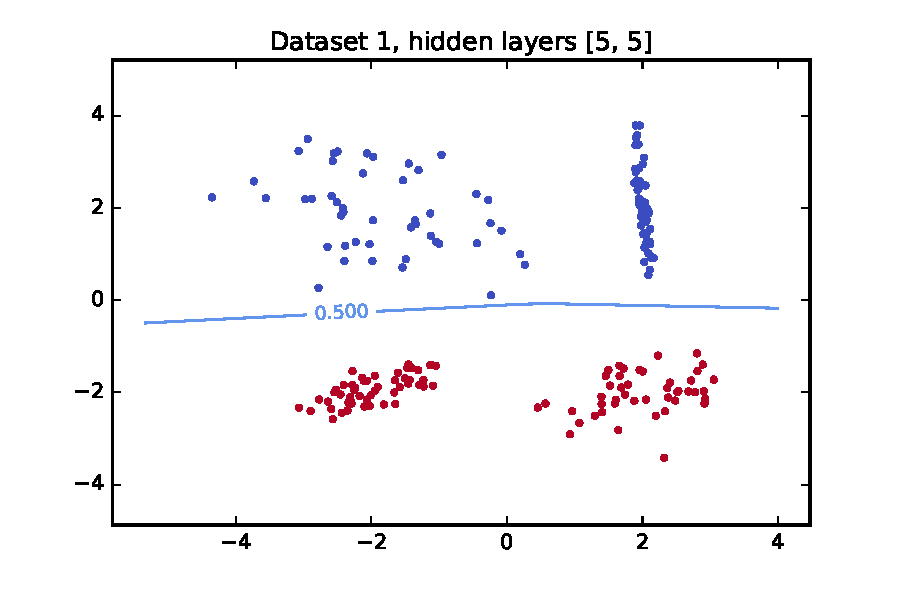
\includegraphics[width=3in]{img/p1/1-200of200.pdf}\hspace{-.25in}
   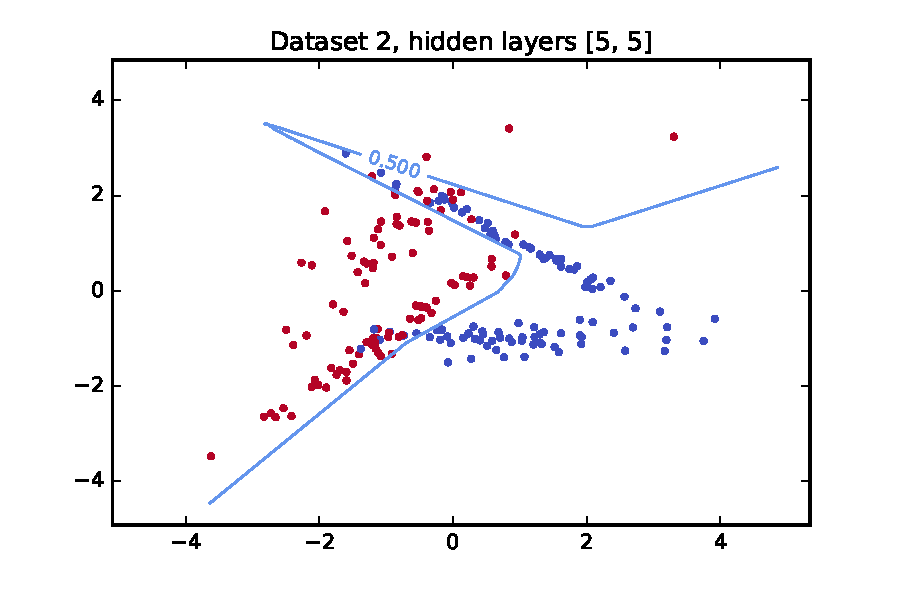
\includegraphics[width=3in]{img/p1/2-183of200.pdf}
   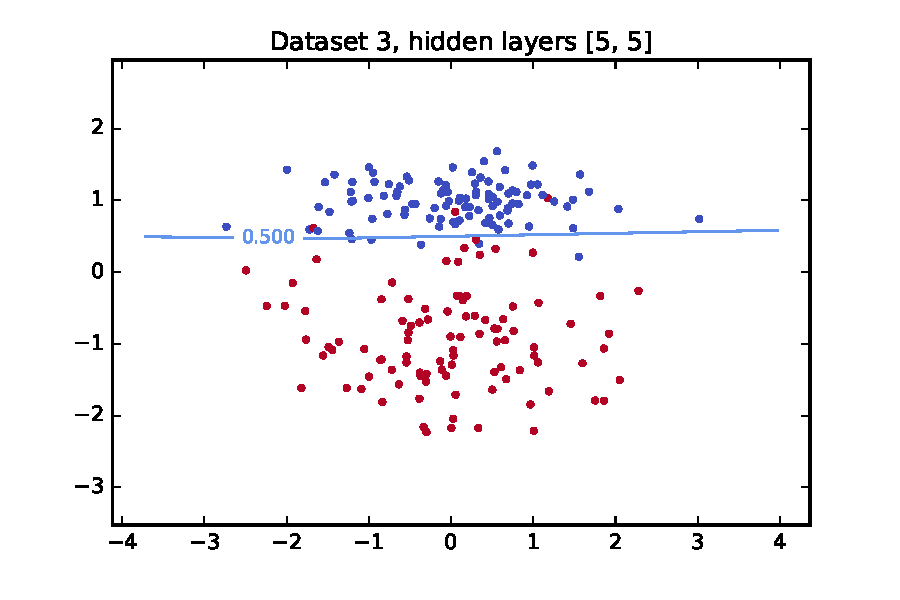
\includegraphics[width=3in]{img/p1/3-192of200.pdf}\hspace{-.25in}
   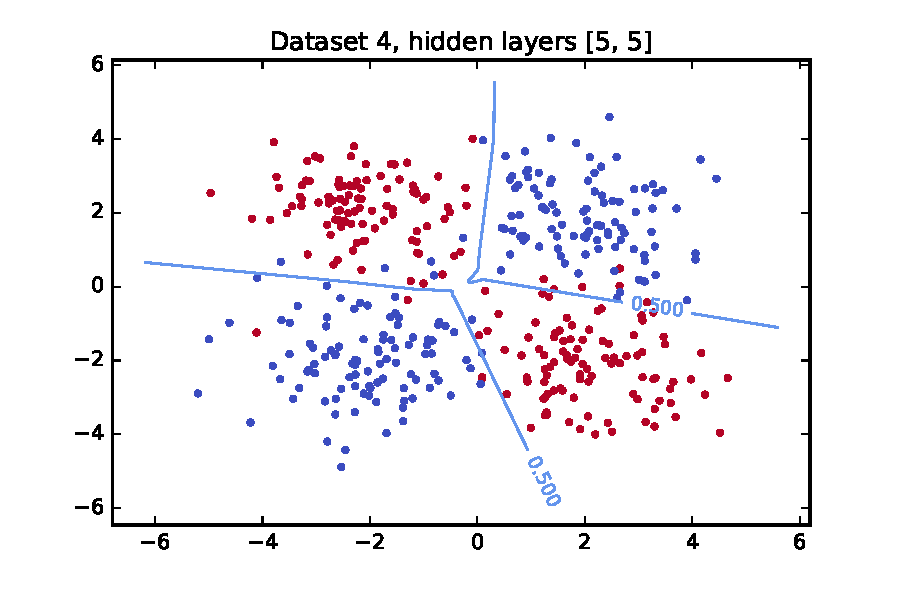
\includegraphics[width=3in]{img/p1/4-382of400.pdf}
   \caption{Neural network classification of four 2D datasets.
   Datasets 1-4 had training/testing accuracies 1.0/1.0, 0.9375/0.915, 0.9825/0.965, and 0.96/0.955,
   respectively.
   }
   \label{fig:1-2-classify}
\end{figure*}

\begin{figure*}
   \centering
   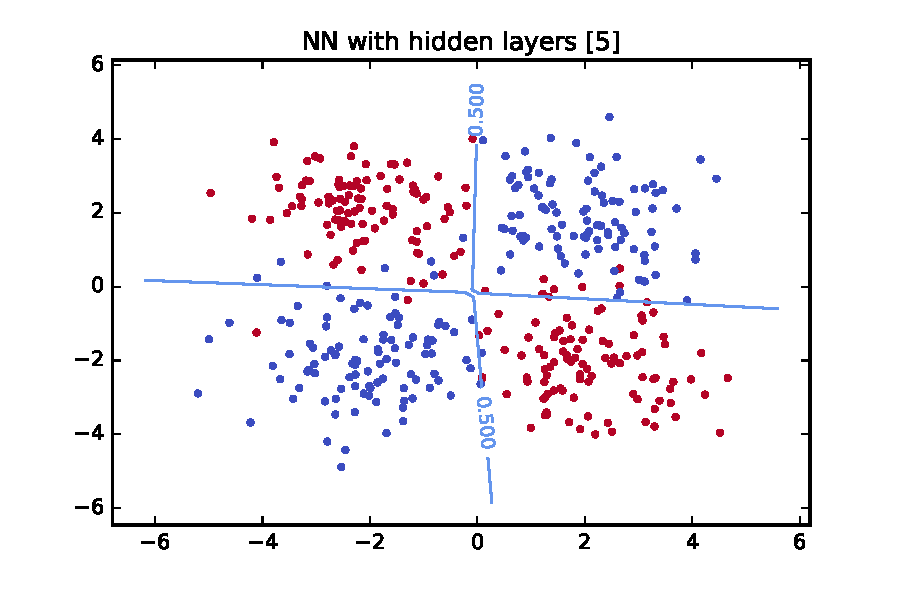
\includegraphics[width=3in]{img/p1/4-1small-382of400-16500.pdf}\hspace{-.25in}
   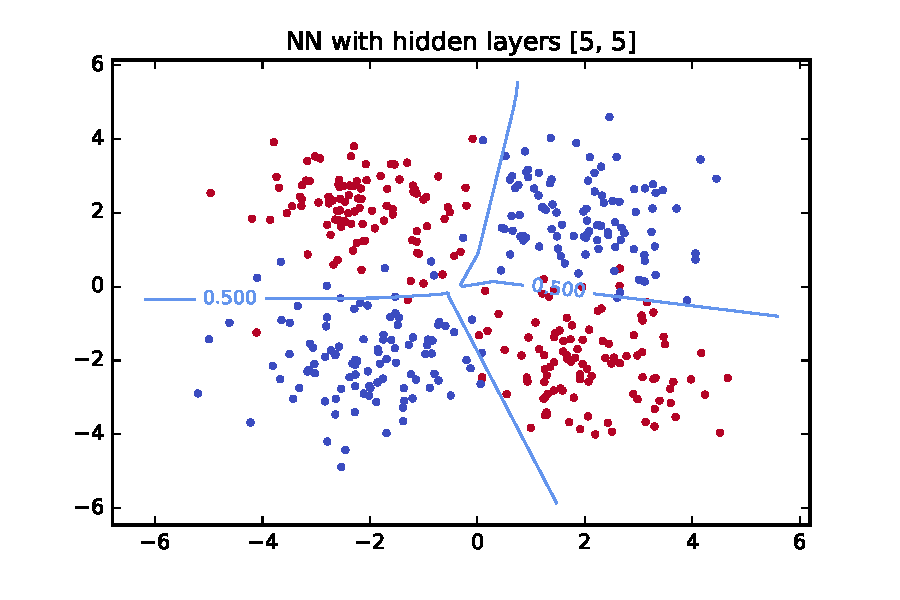
\includegraphics[width=3in]{img/p1/4-2small-380of400-3550.pdf}
   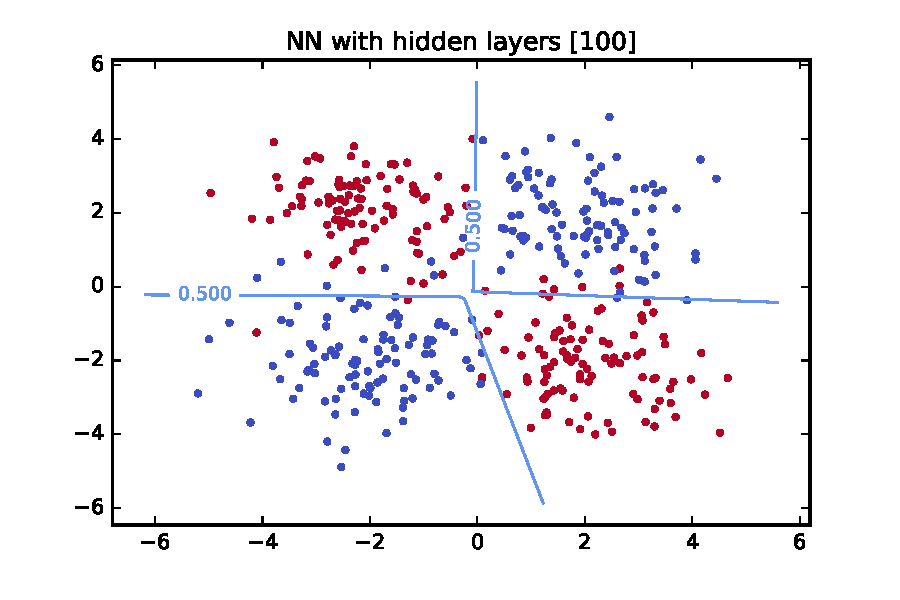
\includegraphics[width=3in]{img/p1/4-1large-380of400.pdf}\hspace{-.25in}
   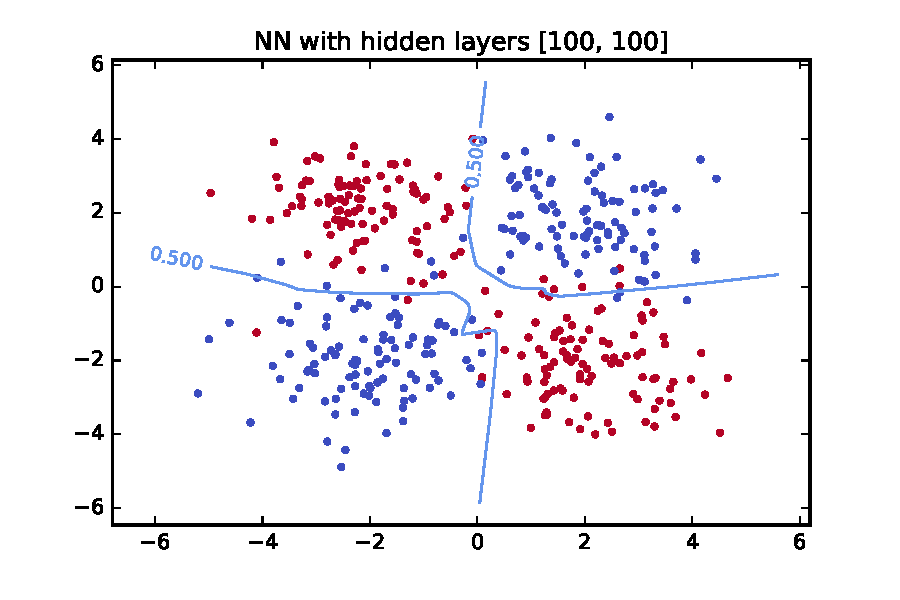
\includegraphics[width=3in]{img/p1/4-2large-379of400-123000.pdf}
   \caption{Variations on neural network architectures for classification of
   XOR data. We see that increasing number of layers increases non-linearity,
   while increasing number of nodes per layer increases overfitting. 
   }
   \label{fig:1-2-arch}
\end{figure*}

\subsection{Network training}

We stochastically updated our weights,
by randomly selecting a sample $(x^{(i)}, y^{(i)})$ per epoch
and updating accordingly.
Our update function is as follows,
\begin{align}
W_{t+1} &= W_t - \eta \f{\partial l}{\partial W_t^l}
= W_t - \eta a^{l-1} (\delta^l)^T \\
b_{t+1} &= b_t - \eta \f{\partial l}{\partial b_t^l}
= b_t - \eta \delta^l
\end{align}
where $l$ is cross-entropy loss, $\eta$ is the learning rate,
and $\delta$ is the calculated backpropagation error.

\subsubsection{Initialization}

Since ReLU is not fully differentiable,
we set the subgradient at 0 to 0.
As a result, we cannot simply initialize weights to 0,
else gradients and activations
will not be updated during training.
Instead, we initialize weights randomly,
with values drawn from a Gaussian centered at 0,
with standard deviation $1/\sqrt{m}$
for a weight matrix of size $m\times n$.

To understand the rationale behind this method,
imagine that all units are sigmoids,
with activation function $f(z) = \f{1}{1+e^{-z}}$.
If weights are too small, then the activations will decrease every layer.
This is an issue since the sigmoid function is approximately linear around 0,
at which we lose the non-linearity of our hidden layers.
However, if our weights are too large,
then the activations will increase indefinitely,
at which point the sigmoid levels off,
and gradients artificially approach 0.
Thus, we want to maintain a constant variance in gradients between
inputs and outputs, such that
\begin{equation}
\f{\sigma^2(z)}{\sigma^2(x)} = \f{\sigma^2(W^TX)}{\sigma^2(X)}
= \f{n\sigma^2(W)\sigma^2{X}}{\sigma^2(X)} = n\sigma^2(W) = 1
\end{equation}
For backpropagation, we use the same logic to derive that
$\sigma^2(W) = 1/m$, so $\sigma(W) = 1/\sqrt{m}$.

\subsubsection{Regularization}

To avoid overfitting, we can add a penalty term to our loss function for regularization.
Our loss would thus become
\begin{equation}
    J(w) = l(w) +
      \lambda
        \lt(\lVert w^{(1)} \rVert^2_F + \lVert w^{(2)} \rVert^2_F\rt)
\end{equation}
where $\lVert w\rVert = \sqrt{\sum_{i,j}{w_{ij}^2}}$ is the Frobenius norm.
In particular, the regularization term is added to the output error $\delta^L$
during backpropagation. The change in $\delta^L$ is then propagated
through to subsequent error calculations for each hidden layer
(even though we don't compute the error again).
Regularization helps prevent weights from becoming too large,
so the neural network will overfit less.

\subsection{Binary classification}
\label{subsubsec:binary}

We tested our implementation against 2D artificial datasets.
The first three contained 400 training samples,
200 validation samples,
and 200 testing samples, and fourth contained 
400 training, validation, and testing samples.
The data consisted of two-dimensional vectors $x\sind{i}$
labeled by $y\sind{i} = \pm1$.
To compare the target values against our softmax outputs,
we mapped $\pm1$ to one-hot vectors $[1,0]$ and $[0,1]$.
Our results are illustrated in Figure~\ref{fig:1-2-classify},
with training and testing accuracies denoted.

We trained our neural network with stochastic gradient descent, with a 
fixed stepsize, $\eta = 0.01$. Stochastic gradient descent terminated when
the change in cross-entropy loss on our validation set dropped below a constant threshold of 0.001.
This loss was calculated once every 100 epochs.

\subsubsection{Architecture variations}
\label{subsubsec:binaryarch}

We investigated different architectures for the neural network,
with varying number of layers and nodes per layer.
Figure~\ref{fig:1-2-arch} illustrates the effect
of these architectures for the classic XOR dataset.
We observed that a single 5-node hidden layer
performed comparably to more complex structures,
while the two 100-node layer network performed the worst, due to overfitting.

We compared our neural network's performance to that of 
logistic regression and a kernelized Gaussian RBF SVM classifier.
Our neural network achieved comparable performance in accuracy,
using optimal parameters for all classifiers,
and two 5-node hidden layers for the neural network.
Our classification accuracies are shown below.

\begin{center}
    \begin{tabular}{c|c|c|c}
        dataset & LR & SVM & NN  \\\hline
        1	&1.0	& 1.0 & 1.0\\
        2	&0.81	& 0.94 & 0.92 \\
        3	&0.975 	& 0.965 & 0.96 \\
        4	&0.50	& 0.9575 & 0.945
    \end{tabular}
\end{center}

\subsection{MNIST multi-class classification}

We also used our neural network to perform multi-class classification of the
MNIST dataset. These data consist $28\times 28$ grayscale images of handwritten
digits, 0 to 9, given as a labeled dataset of $28^2$ dimensional vectors
with integer entries $[0,255]$ representing the grayscale luminescence of each pixel.

We normalized input pixel features to the range $[-1, 1]$,
so that an input vector $x$ is mapped to $\f{2x}{255}-1$,
with all operations applied componentwise.
Normalization significantly improved prediction accuracy.
Class labels were mapped to one-hot vector representations.
For example, an image labeled 9 would have a 
target vector of $[0,0,0,0,0,0,0,0,0,1]$.
We selected 400 training, 200 validation, and 200 testing samples per class.

As in Section \ref{subsubsec:binary}, we determined the termination criteron as
when the change in objective function (cross-entropy loss on softmax output)
dropped below a constant threshold, 0.001 (checked every 500 epochs).

\subsubsection{Architecture variations}

We classified our data with different architectures,
varying number of layers and nodes per layer.
This is analogous to section~\ref{subsubsec:binaryarch}.

% 20,20
%Ran for 302500 iterations.
%Guessed 1851 correct out of 2000 (0.9255)
%Average loss 0.5390193224725606

% 20
%Ran for 216000 iterations.
%Guessed 1876 correct out of 2000 (0.938)
%Average loss 0.6027523211225306

\begin{center}
    \begin{tabular}{c|c|c|c}
        hidden layers & accuracy	& epochs & $\eta$ \\\hline
        20		& 0.9350 	& 216 000 	& 0.01\\
        20,20	& 0.9255 	& 302 500 	& 0.01\\
        100		& 0.9445 	& 152 500 	& 0.01 \\
        100,100	& 0.9505 	& 104 500 	& 0.01
    \end{tabular}
\end{center}

% 4,9 [100]
%Ran for 16500 iterations.
%Guessed 381 correct out of 400 (0.9525)
%Average loss 0.12142020187035087

% 4,9 [100,100]
%Ran for 18000 iterations.
%Guessed 381 correct out of 400 (0.9525)
%Average loss 0.20364621990226375

% 3,5 [100]
%Ran for 10000 iterations.
%Guessed 388 correct out of 400 (0.97)
%Average loss 0.09079234230339693

% 3,5 [100, 100]
%Ran for 13000 iterations.
%Guessed 389 correct out of 400 (0.9725)
%Average loss 0.11671382468804836

% 1,7 [20, 20]
%Ran for 6500 iterations.
%Guessed 394 correct out of 400 (0.985)
%Average loss 0.044168742106228315

% 1,7 [100]
%Ran for 2000 iterations.
%Guessed 397 correct out of 400 (0.9925)
%Average loss 0.03602293463505232

% 1,7 [100, 100]
%Ran for 5500 iterations.
%Guessed 398 correct out of 400 (0.995)
%Average loss 0.029611779980850093

% % % % % % % % % %
%    PROBLEM 2
% % % % % % % % % %

In addition to $k$-class classification of individual digits,
we also used our neural network for binary classification of digit pairs,
to compare with other binary classification methods
(including logistic regression, a linear SVM,
and a SVM with a Gaussian RBF kernel).
For the neural network, we used two 100-node hidden layers,
and the results are below.

\begin{center}
    \begin{tabular}{c|c|c|c|c}
        problem		& NN	& LR		& linear SVM	& RBF kernel \\\hline
        1, 7 & 0.995 	& 0.99 	& 0.986		& 0.986 \\
        3, 5 & 0.9725 	& 0.94 	& 0.946		& 0.983 \\
        4, 9 & 0.9525 	& 0.96 	& 0.943 		& 0.946 \\
    \end{tabular}
\end{center}
The neural network had similar accuracy as the methods under comparison.

\section{Convolutional Neural Networks}

% TODO connect from previous section
% you can connect straight from MNIST cuz images

Empirically, deeper convolution networks work better.
To see why, we introduce the notion of \emph{receptive field}
of a node (a ``pixel" in a feature map):
the pixels from the original image that contribute information
to the node.

% What are the dimensions of the receptive field for a node in Z2?
For example,
suppose we have a convolutional network
with two successive convolutional layers,
with respective patch sizes $5\times 5$ and $3\times 3$.
Each layer has a single feature map (which we name $Z_1$ and $Z_2$).
Then the nodes in $Z_1$ each have $5\times 5$ receptive fields.
Nodes in $Z_2$ will have $(3 + 5 - 1)^2 = 7\times 7$ receptive fields.

% Thinking about your answer,
% why is it effective to build convolutional networks deeper
% (i.e. with more layers)?
In general,
nodes in deeper layers will have larger receptive fields,
so intuitively,
deeper convolutional networks should better detect large-scale structure.

% How many layers are there?
We tested an existing four-layer convolutional network implementation
on an image classification problem,
where given RGB images of 451 paintings by 11 artists
(all downsampled to $50\times 50$),
we would like to predict the artist that painted the given image.

% Are they all convolutional?
% If not, what structure do they have?
The first two layers are convolutional;
each produces 16 feature maps
with $5\times 5$ filters and stride $2$.
We zero-pad the feature maps prior to convolution
so that feature maps remain the same size ($50\times 50$).

Our last two layers are fully connected.
The third layer has 64 hidden units;
the final layer (our output) has 11 units,
corresponding to the 11 artists represented in our dataset.

% Which activation function is used on the hidden nodes?
The network applies a ReLU activation on all hidden nodes.

% What loss function is being used to train the network?
% How is the loss being minimized?
We train the network by minimizing softmax cross-entropy
through minibatch gradient descent,
with batches of 10 examples each.
Recall that average softmax cross-entropy is defined
for labeled examples $(x\sind{i}, y\sind{i})$
(where $y\sind{i}$ is a one-hot vector indicating the category of the example)
as
\begin{equation}
    H(y, \hat y) = \f{1}{n}\sum_{i=1}^n
                             \sum_{j=1}^k
                               y\sind{i}_j \log \hat y\sind{i}_j,
\end{equation}
where $\hat y\sind{i}$ is the prediction made by our network,
a vector of probabilities
produced by applying a softmax function
to the values on our output layer.
For instance, for our image classification problem,
$n$ is the number of images we are evaluating our network on,
and $k=11$ is the number of classification categories.

% What is the training accuracy for your network after training?
% What is the validation accuracy?
% What do these two numbers tell you about what your network is doing?
After 1500 training steps with step size $\eta = 0.01$,
our convolutional network obtains perfect training accuracy,
but only $67\%$ validation accuracy,
strongly suggesting that our network is overfitting.

\subsection{Pooling}

% and choose different values for the pooling filter size and stride.
% After you applied max pooling, what happened to your results?
% How did the training accuracy vs. validation accuracy change?
We modified our network by adding max-pooling
after both convolutional layers.
We experimented with various pooling filter sizes (1 to 4)
and strides (1 to 4).
In all cases,
pooling modestly reduced training accuracy
(from around $100\%$ to $90\%$),
but did not improve validation accuracy noticeably.
Accuracy was typically $60\%$ to $70\%$.

Variations in validation accuracy
stemmed from the randomness inherent in our stochastic training scheme,
as variation in accuracy between runs with different hyperparameters
was comparable to the that between runs with the same hyperparameters.
% make less verbose?

% What does that tell you about the effect of max pooling on your network?
We conclude that max-pooling provides little improvement
to our convolutional network's accuracy.
We do note, however, that overfitting was reduced,
since training accuracy matched validation accuracy more closely.

\subsection{Regularization}

To combat the overfitting we saw earlier,
we tested various methods of regularization.
Unless otherwise stated,
in each section we \emph{only} vary the hyperparameter in question;
we leave the remaining hyperparameters (e.g. training steps, pooling) unchanged.

% Test each one individually,
% and discuss how it affects your results.

\subsubsection{Dropout}


We implemented dropout for the fully connected layer (the third layer).
We tested various values of dropout parameter~$p$,
the probability we do \emph{not} drop out a neuron.
For each $p$, we trained $n=10$ separate models;
we present the mean training and validation accuracies
with their respective standard errors here.
Training accuracies are quoted on the final minibatch of ten samples.
\begin{center}
    \begin{tabular}{c|cc}
        $p$ & Train $\pm 1 \sigma$ (\%) & Validation $\pm 1 \sigma$\\\hline
        0.6 &  $77.00 \pm 2.60$ & $62.18 \pm 0.81$ \\
        0.7 &  $75.00 \pm 3.42$ & $62.53 \pm 0.86$ \\
        0.8 &  $89.00 \pm 3.48$ & $65.52 \pm 1.24$ \\
        0.9 &  $94.00 \pm 2.21$ & $65.63 \pm 0.55$ \\
        1.0 & $100.00 \pm 0.00$ & $65.63 \pm 1.01$ \\
    \end{tabular}
\end{center}

% You should explore different values of dropout_prob
% to find one that works well.
While dropout reduces training accuracy significantly,
it only modestly affects validation accuracy.
So while dropout combats overfitting,
it doesn't improve our model's ability to generalize.

We also tested dropout together with pooling;
validation accuracies were slightly, but noticeably lower.


\subsubsection{Weight regularization}

As we did previously,  % TODO check that this is mentioned in previous section
we experimented with adding a regularization term
to our training loss.
In particular, we modify our softmax cross-entropy loss $\ell(w)$
to get a new loss
\begin{equation}
    \ell(w) + \lambda\sum_i \lVert w\sind{i} \rVert^2
\end{equation}
where we include an extra term:
the sum of the squared Frobenius norms of the weight matrices $w\sind{i}$
of the two fully-connected layers,
weighted by a regularization parameter~$\lambda$.

Again, we test each value of $\lambda$ ten times,
and present the mean accuracies (with associated standard errors) below.

\begin{center}
    \begin{tabular}{c|cc}
        $\lambda$ & Train $\pm 1 \sigma$ (\%) & Validation $\pm 1 \sigma$\\\hline
        0    & $100.00 \pm 0.00$ & $65.40 \pm 1.19$ \\
        0.01 & $100.00 \pm 0.00$ & $66.44 \pm 1.15$ \\
        0.03 & $100.00 \pm 0.00$ & $66.55 \pm 0.76$ \\
        0.1  & $100.00 \pm 0.00$ & $65.40 \pm 0.81$ \\
        0.3  &  $79.00 \pm 2.33$ & $52.64 \pm 1.36$ \\
      % 1.0  &  $50.00 \pm 0.00$ & $37.70 \pm 0.33$ \\
    \end{tabular}
\end{center}
Small values of $\lambda$ produced
statistically insignificant improvement in validation accuracies;
larger values saw significantly worse performance
in both training and validation accuracies.
Thus, weight regularization
is unlikely to be particularly helpful.


\subsubsection{Data augmentation}

We next enlarged our training dataset
with transformed versions of the original training samples
and trained on this augmented dataset.
This new dataset was four times as large as the original,
so we quadrupled the number of training steps
when working with the augmented training data.

We present our results as below.
As before, we repeat training ten times
and report means and standard errors.
\begin{center}
    \begin{tabular}{cc|cc}
        Aug. & Steps & Train $\pm 1 \sigma$ (\%) & Validation $\pm 1 \sigma$\\\hline
        No  & 1500 & $100.00 \pm 0.00$ & $65.98 \pm 1.03$ \\
%        No  & 6000 & $100.00 \pm 0.00$ & $66.21 \pm 0.86$ \\
        Yes & 6000 & $100.00 \pm 0.00$ & $62.30 \pm 0.61$
    \end{tabular}
\end{center}

Note that data augmentation actually lowered our validation accuracy.
Indeed, using the augmented data with 6000 steps
produced statistically significantly worse results
than using the original training set with 1500 steps
(Student's $t$-test, $p=0.0066$).

\subsubsection{Early stopping}

Finally, we consider early stopping as a means of regularization.
We monitored the validation error
of our model each time we trained it;
we show a representative plot in Figure~\ref{fig:2-4-4-validation-acc}.

\begin{figure*}[t]
   \centering
   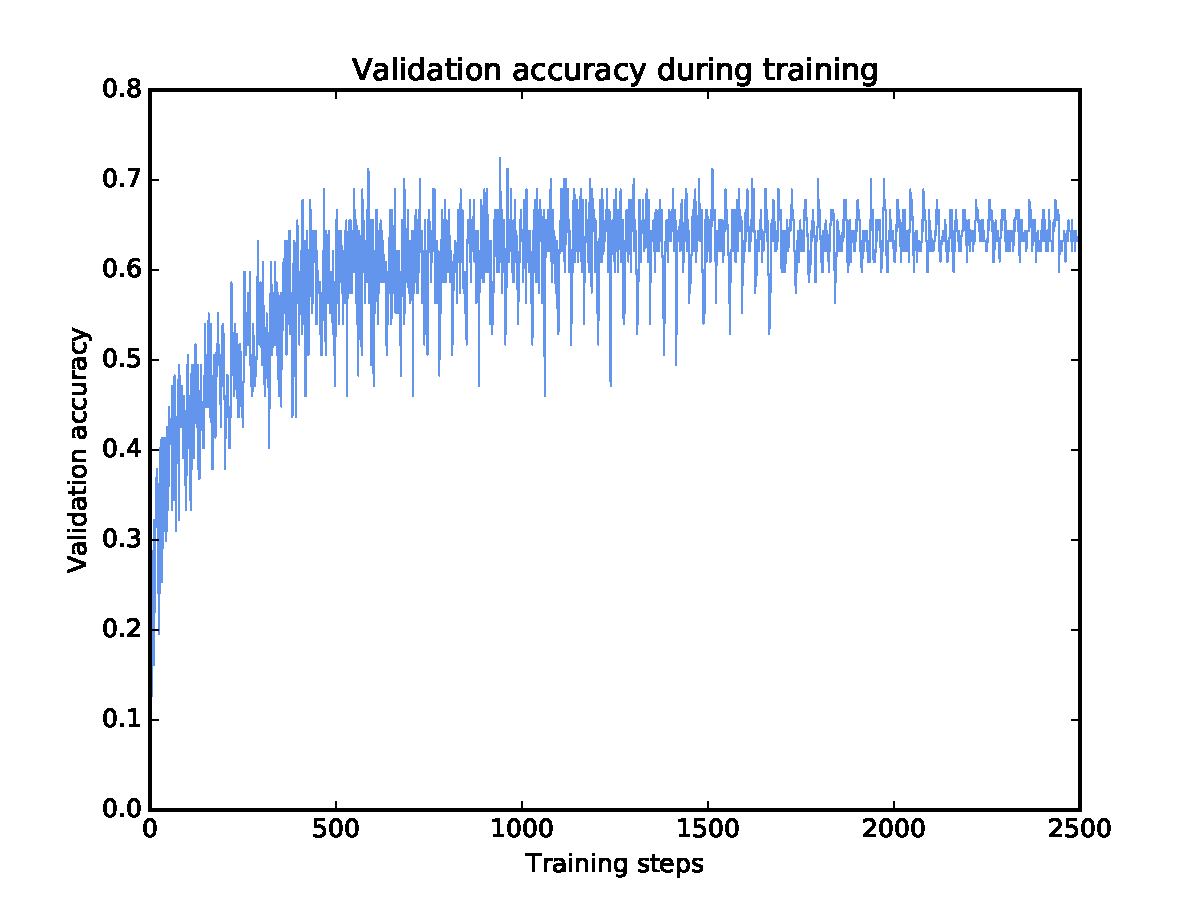
\includegraphics[width=4in]{img/2-4-4-validation-acc-new.pdf}
   \caption{Validation error of our convolutional network during training.}
   \label{fig:2-4-4-validation-acc}
\end{figure*}

After around 1000 training steps,
validation accuracy fails to improve further.
We note, however, that validation accuracy
does not significantly \emph{decrease}
as we continue to train our model,
suggesting that overfitting (if it is occurring at all)
is not negatively impacting our results.

In summary, none of our regularization schemes
was particularly effective in improving validation accuracy.



\subsection{Architectural variations}

We also experimented with varying our network architecture,
rather than just with training parameters
(e.g. weight regularization, dropout).

%    Report which changes led to
%    the biggest increases and decreases in performance.
%    In particular,
%    what is the effect of making the convolutional layers have
%    a) a larger filter size,

\subsubsection{Filter sizes}

We tested larger and smaller filter sizes
on each convolutional layer.
We first tried changing the filter sizes on both layers simultaneously,
leaving other hyperparameters fixed.
Our results show that filters larger than $5\times 5$
work just as well,
while smaller filters perform significantly worse.

We also tried more novel filter size combinations.
None yielded any statistically significant improvement
over our original $5\times 5$ filters.

%We present some of our findings
%in Figure~\ref{fig:filter-size-experiment}.
%
%\begin{figure*}[t]
%   \centering
%   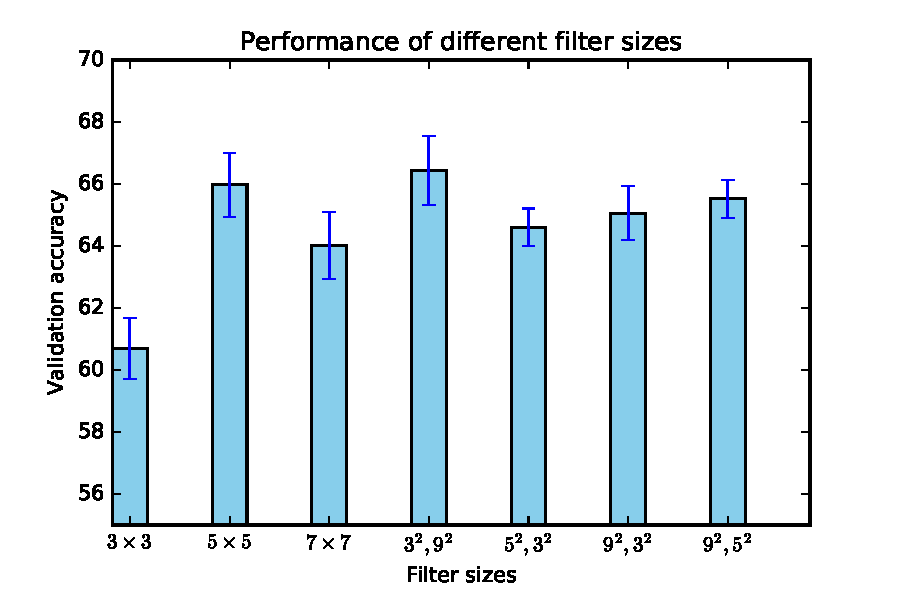
\includegraphics[width=4in]{img/2-5-filter-size-acc.pdf} 
%   \caption{Mean validation accuracies for various filter size choices (each tested $n=10$ times).
%       Error bars denote standard error of the mean.}
%   \label{fig:filter-size-experiment}
%\end{figure*}

%\begin{center}
%    \begin{tabular}{c|cc}
%        Filter sizes & Train $\pm 1 \sigma$ (\%) & Validation $\pm 1 \sigma$\\\hline
%        $3\times 3$ & $95.00 \pm 1.67$ & $60.69 \pm 0.98$ \\
%        $5\times 5$ & $100.00 \pm 0.00$ & $65.98 \pm 1.03$ \\
%        $7\times 7$ & $100.00 \pm 0.00$ & $64.02 \pm 1.07$ \\
%        $3^2$ then $9^2$ & $100.00 \pm 0.00$ & $66.44 \pm 1.12$ \\
%        $5^2$ then $3^2$ & $98.00 \pm 2.00$ & $64.60 \pm 0.61$ \\
%        $9^2$ then $3^2$ & $100.00 \pm 0.00$ & $65.06 \pm 0.88$ \\        
%        $9^2$ then $5^2$ & $100.00 \pm 0.00$ & $65.52 \pm 0.62$
%    \end{tabular}
%\end{center}


\subsubsection{Stride}

%    b) a larger stride and
We tried varying the strides on our convolution100
al layers as well.
No setting we tried yielded statistically significant improvement
over our baseline $5\times 5$ filters with stride $2$.


%    c) greater depth?
\subsubsection{Depth}

Finally, we considered the number of feature maps
we used at each layer.
For this section,
we including $2\times 2$ max-pooling layers with stride 2
after each convolutional layer.

Holding the depths of the convolutional layers
equal to each other,
we find that increasing the depth has a significant positive effect
on validation accuracies,
as is evident from Figure~\ref{fig:2-5-conv-depth-val-acc}.
For instance, at depth 45,
we achieved a mean validation accuracy of $70.46 \pm 0.91\%$,
which was statistically significantly greater
than our baseline at depth~15 of $64.83 \pm 1.11\%$
(Student's $t$-test, $p=0.001$).

\begin{figure*}[t]
   \centering
   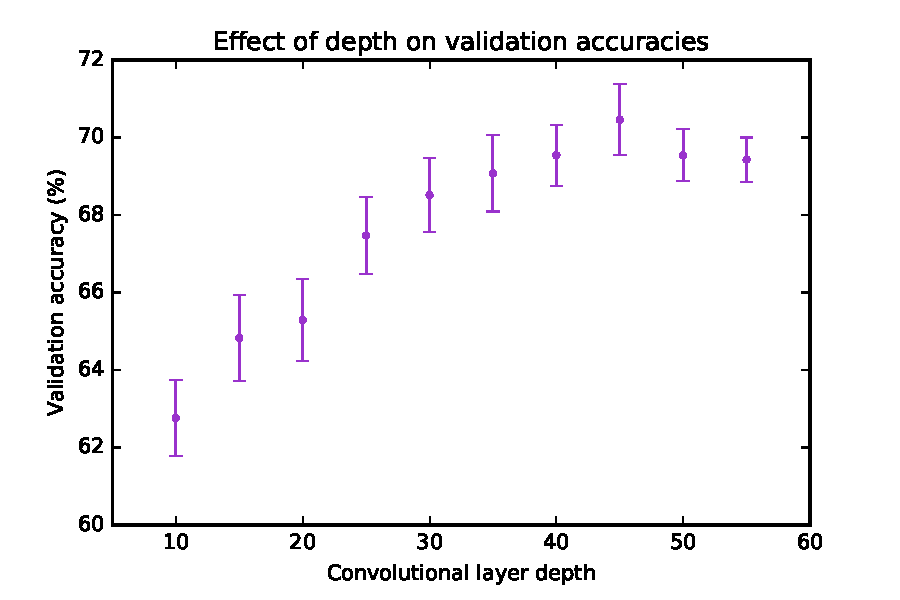
\includegraphics[width=4in]{img/2-5-conv-depth-val-acc.pdf}
   \caption{Mean validation accuracies (with standard errors of the means)
       of convolutional networks with equal depth at both convolutional layers.}
   \label{fig:2-5-conv-depth-val-acc}
\end{figure*}

The training accuracy was close to perfect
for each of these tests,
suggesting some degree of overfitting.


%    How does a pyramidal-shaped network
%    in which the feature maps gradually decrease in height and width
%    but increase in depth
%    compare to a flat architecture,
%    or one with the opposite shape?

We also varied depths independently.
In particular,
we tested ``pyramidal" architectures
in which we gave the second layer a larger depth
compared with the first.
Of course, we also tried the inverse architecture,
with smaller depths on the second layer.
No such architecture performed better
than the best architecture we found when
we varied the depths in lockstep (depths 45 and 45).



\end{multicols}

\end{document}



